\chapter{Mise en place du protocole de communication}
	Le premier chapitre de se rapport a présenté les principales idées que l'on souhaite mettre en 
	place pour avoir une architecture d'objets dynamique et générique. On va maintenant s'intéresser
	à la manière dont on peut les réaliser.


\section{Les protocoles existants}
	Il existe une multitude de supports de communication déjà existants, dont les plus connus sont 
zigbee, et zwave dans le milieu de la domotique. Il existe une autre alternative qui commence à arriver qui 
s'appelle AllJoyn qui seront expliqués après.

	\subsection{Zigbee}
	ZigBee est un protocole de haut niveau permettant la communication, à basse consommation. Ce 
protocole est basé sur la norme IEEE 802.15.4 et est utilisée pour les réseaux WPAN (\emph{Wireless Personal 
Area Networks}). Le principal avantage de ce support est sa capacité à créer réseau maillé dynamique et 
autonome, ce qui est très pratique pour créer un réseau d'objet dynamique.

	\subsection{Z-Wave}
	Z-wave est un protocole qui ressemble beaucoup au zigbee. En effet lui aussi permet de créer un 
réseau maillé dynamique. Les quelques différences avec le z-wave sont principalement :

\begin{itemize}
 \item Les bandes de fréquences : 868 MHz, 915 MHz et 2.4 GHz pour le ZigBee; 868 MHz et 908 MHz pour le 
Z-Wave
\item Le nombre de noeuds dans le réseau : 232 pour Z-Wave et 64000 pour ZigBee.
\end{itemize}

	\subsection{Alljoyn}
	Alljoyn est un projet open source international, porté par Qualcomm et présenté pour la première fois 
en 2011. Ce protocole a pour but de communiquer avec tous les objets autour en s'abstrayant du support de 
communication, et en étant compatible avec tous les systèmes du marchés
	% A ECRIRE, A ECRIRE	, A ECRIRE, A ECRIRE, A ECRIRE, A ECRIRE
	
	% IMPORTANT : explication de pourquoi on a pas pris un protocole existant :
	%  - ne correspond pas forcément à toute les fonctionnalités que l'on souhaite mettre en place
	%  - est difficilement adaptable avec les outils que l'on a (mbed, attiny, bluetooth Bolutek)

\section{Le réseau virtuel}
	Nous allons maintenant nous intéresser aux caractéristiques du protocole qui a été
	développé dans ce projet. L'un des points clés de la mise en place d'objets pour la domotique 
	est la communication avec ceux-ci. Ces objets doivent en effet être "connectés" pour que l'on
	puisse les contrôler ou recevoir des messages de leur part. Il est donc nécessaire de mettre en 
	place une architecture réseau qui puisse lier ces objets de façon efficace. Mais la mise en place
	de ce réseau n'est pas forcément évidente. Si l'on souhaite être indépendant du support de 
	communication, il faut mettre en place des moyens de lier des objets de supports différents. Il 
	est également possible de communiquer avec des objets mobiles. Cela signifie que l'architecture 
	du réseau doit également être dynamique. C'est pourquoi il est indispensable d'avoir un protocole
	capable de gérer tous ces détails.
	
	\subsection{Architecture du réseau}
% 		définition d’un réseau (uniquement 1 support de communication)
% 		description de la connexion des réseaux
% 		exemples d’architecture de réseau virtuel
		Pour bien comprendre comment est structuré un réseau d'objets, il faut d'abord s'intéresser 
		à une architecture simple ne faisant qu'intervenir un seul support de communication. La figure
		\ref{netStar} représente un réseau créé par des objets connectés possédant une interface Wifi.
		En utilisant du Wifi \emph{Point d'Accès}, un des objets fait office de serveur (\emph{C}) 
		sur lequel les autres objets clients viendront se connecter. Avec cette architecture de 
		réseau, l'ensemble des objets peuvent parler entre eux mais tous les messages passent par 
		\emph{C}. Cette connexion est complètement transparente à l'utilisation puisqu'elle 
		directement gérée par le protocole IP. La communication consistera simplement à créer une
		\emph{socket} TCP ou UDP entre deux objets. Ils pouront alors parler sans avoir à s'occuper
		du transport de leurs messages.
		
		\begin{figure}[!ht]
         \centering
         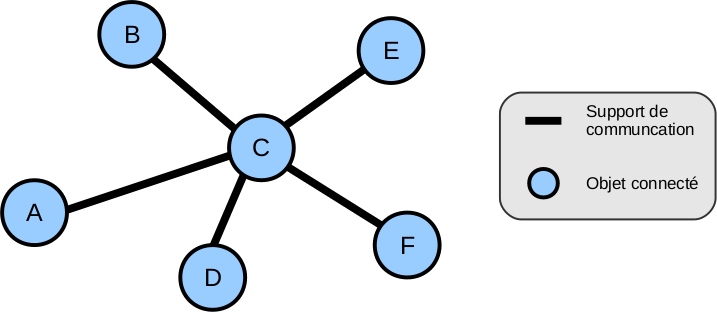
\includegraphics[width=.8\textwidth]{img/reseau_etoile.png}
         \caption{Exemple d'architecture réseau d'un point d'accès Wifi (topologie en étoile).}
         \label{netStar}
      \end{figure}

      Si l'on prend cette fois-ci l'exemple d'une architecture formée par d'objets utilisant 
      ZigBee (figure \ref{netGraph}), on remarque que les objets ne sont pas lié à un unique objet
      mais à l'ensemble des objets qui sont à sa portée. Un objet peut donc communiquer directement
      avec un objet voisin mais également avec des objets plus distants s'il existe un chemin dans
      le graphe du réseau. Encore une fois, toute cette architecture est déjà gérée nativement par
      les composants ZigBee. Cependant son utilisation est un peu différente d'une utilisation 
		d'objets en Wifi. Certains protocoles de communication utilisant du ZigBee (par exemple Xbee) 
		ne permettent pas d'envoyer des messages à une cible précise. C'est la totalité des objets qui
		sont présent dans le réseau ZigBee qui recevront le message. Cela signifie qu'il faudra gérer
		la cible dans le message en lui-même. Cette méthode peut être un inconvénient puisqu'il
		complexifie la création des messages mais il offre un avantage au niveau du transport de ces
		messages.
      
      \begin{figure}[!ht]
         \centering
         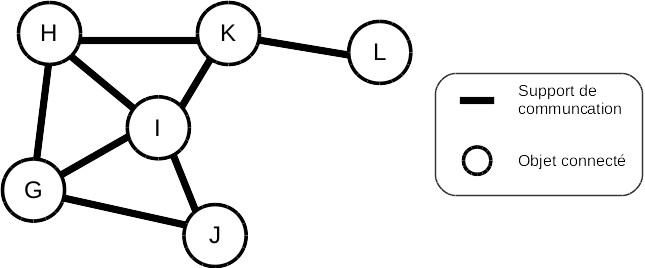
\includegraphics[width=.8\textwidth]{img/reseau_graphe.png}
         \caption{Exemple d'architecture réseau d'objet en ZigBee (topologie en maillage).}
         \label{netGraph}
      \end{figure}
      
      Ces deux architectures sont les plus courantes dans les technologies de communication sans
      fils. Certaines de ces technologies offrent même la possibilité de choisir quelle 
		architecture on souhaite utiliser. En domotique, la plupart des produits proposés dans le
		marché utilise une architecture maillée car elle est la plus adaptée aux tailles des maisons.
		Mais souvent, ces produits nous limitent à l'utilisation d'une même technologie de 
		communication pour tous les objets de la maison (et également de la même marque). Ceci peut
		être problématique lorsque l'on souhaite ajouter dans le réseau un objet connecté que l'on
		aurait fabriqué nous même. En effet, certains de ces produits utilisent des technologies assez
		onéreuses. Une façon de résoudre ce problème est de ne pas limiter le réseau à un unique
		support de communication mais à mettre en place des outils permettant de connecter entre eux
		différents supports.
		
      \begin{figure}[!ht]
         \centering
         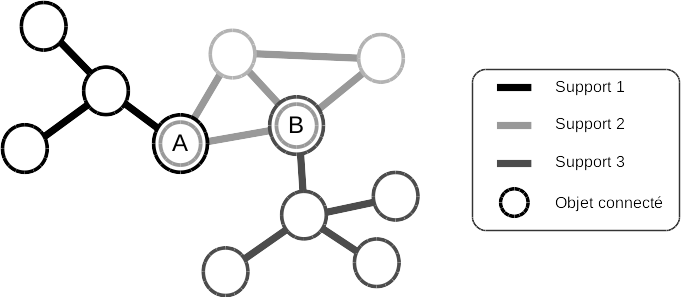
\includegraphics[width=.8\textwidth]{img/multinet.png}
         \caption{Exemple d'architecture réseau mélangeant plusieurs supports de communication.}
         \label{multinet}
      \end{figure}
      
      La figure \ref{multinet} est un exemple de réseau que notre protocole est capable de gérer. On
      peut voir qu'il permet de lier entre eux 3 supports de communication différents ayant 
		également des architectures de réseau différente. Le lien entre chacun de ces supports est
		réalisé par des objets connectés un peu particulier que l'on appelle des \emph{passerelles} 
		(\emph{A} et \emph{B} sur le schéma).
		Ces objets peuvent fonctionner de la même façon que n'importe quel autre objet. Ils ont
		cependant la possibilité de communiquer sur différents supports. Cela signifie que ces objets
		sont équipés au minimum de 2 technologies de communications. Par exemple, Wifi + Bluetooth,
		ZigBee + Ethernet ou même Wifi + Wifi (dans 2 réseaux différents).
		
	\subsection{Le routage}
% 		présentation du protocole VIP
% 		explication du transfert d’un message d’un support à un autre
% 		exemple concret d’un envoi de message
		Même avec une architecture de réseau comme celle de la figure \ref{multinet}, il faut laisser
		la possibilité à chaque objet de pouvoir communiquer avec n'importe quel autre objet. Cela ne
		sera pas aussi simple qu'avec une architecture ne contenant qu'un seul support.
		
		On va considérer que deux objets connectés sont \emph{voisins} s'ils appartiennent au même
		support de communication. On souhaite par exemple que l'objet \emph{C} envoi un message
		à l'objet \emph{F}. La première chose à faire est de déterminer qui est la cible. Étant donné
		que les deux objets appartiennent au même support, il suffit d'utiliser les adresses de 
		support de \emph{F} et\emph{C} (l'adresse MAC pour le Bluetooth, l'adresse IP pour le Wifi, 
		\dots). Le message sera alors
		transmit sans aucun problème puisque ce sera la technologie de communication qui s'occupera 
		du transport du message. Maintenant on souhaite que l'objet \emph{C} envoi un message à 
		l'objet \emph{G}. Cette fois-ci il va y avoir un problème puisque ces deux objets
		n'appartiennent pas au même support. L'utilisation des adresses de support ne servira à rien
		puisqu'elle ne seront pas compatibles. De plus, il est nécessaire de faire intervenir les
		objets \emph{A} et \emph{B} car ils font obligatoirement partie du transport du message.
		
		Ce problème a déjà été abordé lors de la création des premiers réseaux informatiques. Il 
		existe différentes solutions mais la plus connue est sans doute celle qui est actuellement 
		utilisée dans nos ordinateurs : le protocole IP. Cela signifie qu'il faut mettre en place un
		système similaire à celui qui relie les machines du monde entier. L'ensemble des objets
		connectés formera donc un \emph{réseau virtuelle} qui s'appliquera comme une surcouche aux
		technologies de communication existantes. Le nom de ce nouveau protocole des objets connectés
		est \emph{VIP} (Virtual Internet Protocol) imittant de façon simplifiée le protocole IP. Il
		est également accompagné du protocole VARP (virtual adress resolution protocol) qui sera 
		détaillé plus tard.
		
		\subsubsection{Le protocole VIP}
			Le protocole VIP définit pour chacun des objets une adresse VIP qui est composée de 3 
			octets (tableau \ref{vipFormat}). Chacun de ces octets possède une utilité précise. Le
			premier octet est utilisé pour référencer l'adresse du réseau. C'est une adresse globale
			qui sert à regrouper ensemble plusieurs sous-réseaux. En pratique, on utilise la même
			adresse de réseau pour la totalité des objets d'une maison. Cependant, si la maison
			possède plus de 64516 objets, il faudra au minimum 2 adresses de réseau pour représsenter
			une maison. Le deuxième octet de l'adresse VIP représente l'adresse de sous-réseau. C'est
			l'adresse d'un support de communication. Cela signifie que tous les objets d'un même
			support doivent utiliser la même adresse de sous-réseau. Encore une fois, s'il y a plus
			de 254 objets dans le même support, il faudra utiliser plusieurs adresses de support. Mais
			il faudra cependant ajouter des objets passerelles dans le même support pour que tous les
			objets puissent communiquer entre eux. Le dernier octet de l'adresse VIP va enfin définir
			l'adresse de l'objet. Cette adresse doit bien sûr être unique pour chaques objets d'un même
			sous-réseau.
			
			\begin{table}[ht]
				\centering
				\begin{tabular}{|l|l|l|}
					\hline
					Nom                         & Taille (bits) & Description              \\ 
					\hline\hline
					\texttt{ADDR{\_}NET}        & 8             & l'adresse de réseau      \\ \hline
					\texttt{ADDR{\_}SUB{\_}NET} & 8             & l'adresse de sous réseau \\ \hline
					\texttt{ADDR{\_}DEV}        & 8             & l'adresse de l'objet     \\ \hline
				\end{tabular}
				\caption{Format d'une adresse VIP}
				\label{vipFormat}
			\end{table}
			
			Il existe cependant des valeurs particulières d'adresse VIP : 
			\paragraph{Les adresses de réseaux}
				Toutes les addresses VIP dont l'adresse d'objet est 0 représente l'adresse du 
				sous-réseau. Cela signifie que l'adresse de décrit pas un objet mais le sous-réseau 
				lui-même. De la même façon, toutes les adresse VIP dont l'adresse de sous-réseau est 0 
				représente 	l'adresse de réseau (l'adresse doit valoir également 0).
				
			\paragraph{Les adresses de broadcast}
				Une adresse de broadcast est une adresse un peu particulière puisqu'elle représente la
				totalité des objets possédant le même réseau ou sous réseau que l'adresse de broadcast.
				Elle est définie avec la valeur maximale d'un ou plusieurs octets de son adresse VIP.
				Il faut cependant que ces octets soient les derniers de l'adresse.
				
			Les adresses VIP sont donc très similaire aux adresses IP. Elles n'ont cependant pas la
			même flexibilité puisque IP offre la possibilité de définir des masques de sous-réseaux
			dynamiques. Il y a également une différence au niveau de la représentation textuelle d'une
			adresse. Une adresse VIP s'écrit de la façon suivante : \\
			\makebox[\textwidth]{\texttt{ADDR{\_}NET:ADDR{\_}SUB{\_}NET:ADDR{\_}DEV}}
			en remplaçant chaque \texttt{ADDR} par sa valeur en hexadécimal. 
			Le tableau \ref{vipExample} montre quelques exemples d'adresse VIP.

			\begin{table}[!ht]
				\centering
				\begin{tabular}{ll}
					\texttt{0f:34:02} & objet 0x02 du sous-réseau 0x34 du réseau 0x02 \\
					\texttt{aa:b2:27} & objet 0x27 du sous-réseau 0xb2 du réseau 0xaa \\
					\texttt{aa:32:1c} & objet 0x1c du sous-réseau 0x32 du réseau 0xaa \\
					\texttt{23:00:00}	& adresse du réseau 0x23	\\
					\texttt{23:4b:00}	& adresse du sous-réseau 0x4b du réseau 0x23 \\
					\texttt{23:4b:ff}	& adresse de broadcast du sous-réseau précédent \\
					\texttt{23:ff:ff}	& broadcast à tous les objets du réseau 0x23 \\
					\texttt{ff:ff:ff}	& broadcast à tous le monde (à utiliser de faon modérée) \\
					\texttt{00:00:00}	& adresse du réseau virtuel (utile pour le routage) \\
				\end{tabular}
				\caption{Exemples d'adresses VIP.}
				\label{vipExample}
			\end{table}

			Avec ce système d'adresse pour les objets connectés, il est maintenant possible
			d'identifier de façon uniforme chaque objet du réseau virtuel mais également de pouvoir
			gérer la communication entre des objets de supports différents grâce au mécanisme de
			\emph{routage}. En effet, chaque objet est équipé d'une table que l'on appelle
			\emph{table de routage}. Ces tables permettent de définir le chemin que va	prendre un
			message entre un objet \emph{A} et un objet \emph{B}. Elles contiennent une liste 
			décrivant, pour chaque interface de communication d'un objet, l'adresse vers qui envoyer 
			les données en fonction du destinataire du message. Cela signifie que si l'on souhaite
			envoyer un message à une certaine adresse, le programme parcourra la table de routage à la
			recherche de la première règle qui correspondra à l'adresse. Le message sera alors envoyé
			à la passerelle associée la règle correspondante dans la table. Si aucune règle n'est
			adapté, il prendra la règle par défaut (adresse \texttt{00:00:00}). On peut également
			mettre des règles dont l'adresse de passerelle est \texttt{00:00:00}. Cela signifie que
			la passerelle est l'objet lui-même (c'est un réseau local à l'objet).
			
			Pour mieux comprendre ce mécanisme, prenons un exemple dans la figure \ref{vipNet}. L'objet
			\emph{C} souhaite envoyer un message à l'objet \emph{F}. Le tableau \ref{routingTable}
			donne la table de routage de chacun des objets connectés décrits dans la figure. La table
			qui nous intéresse dans cet exemple est celle de l'objet \emph{C} car il faut déterminer
			l'interface de communication qu'il faut utiliser pour émettre le message. Dans le cas de
			cet objet, la solution est vite trouvée puisqu'il ne possède qu'une seule interface :
			le support 1. L'adresse de l'objet \emph{F} est \texttt{01:4b:17}. L'objet \emph{C} va donc
			chercher l'adresse de réseau correspondante. La première ligne de la table concerne le
			réseau d'adresse \texttt{01:4b:00}. Cette ligne est déjà valide pour l'adresse de l'objet
			\emph{F}. Le message doit donc être envoyé à l'adresse de la passerelle de cette ligne.
			Il se trouve que l'adresse de passerelle est l'adresse par défaut. Cela signifie que l'on
			peut envoyer le message directement à l'objet \emph{F}. Il n'y a pas besoin de passer par 
			des intermédiaires.
			
			Maintenant, on va analyser l'envoi d'une message vers une destination plus lointaine.
			Prenons le cas de l'envoi d'un message entre l'objet \emph{C} et l'objet \emph{G}. 
			L'adresse de l'objet \emph{G} est \texttt{01:cc:42}. Dans la table de routage de \emph{C},
			la ligne concerné va être la deuxième puisque le réseau \texttt{01:cc:00} n'est pas connu.
			Il va donc envoyer le message à l'objet \emph{A} (la passerelle). Après réception du
			message par l'objet \emph{A}, celui-ci va lire sa table de routage pour chercher l'adresse
			de \emph{G}. La règle valide pour cette adresse est encore une fois la règle par défaut. Le
			message va donc être envoyer à l'objet d'adresse \texttt{01:e5:33} (l'objet \emph{B}).
			C'est ensuite au tour de \emph{B} de lire sa table de routage. Cette fois-ci le réseau
			\texttt{01:cc:00} est connue. La règle valide dans sa table est donc la deuxième. Le
			message sera ensuite envoyé à l'objet \emph{G}.
			
			\begin{figure}[!ht]
				\centering
				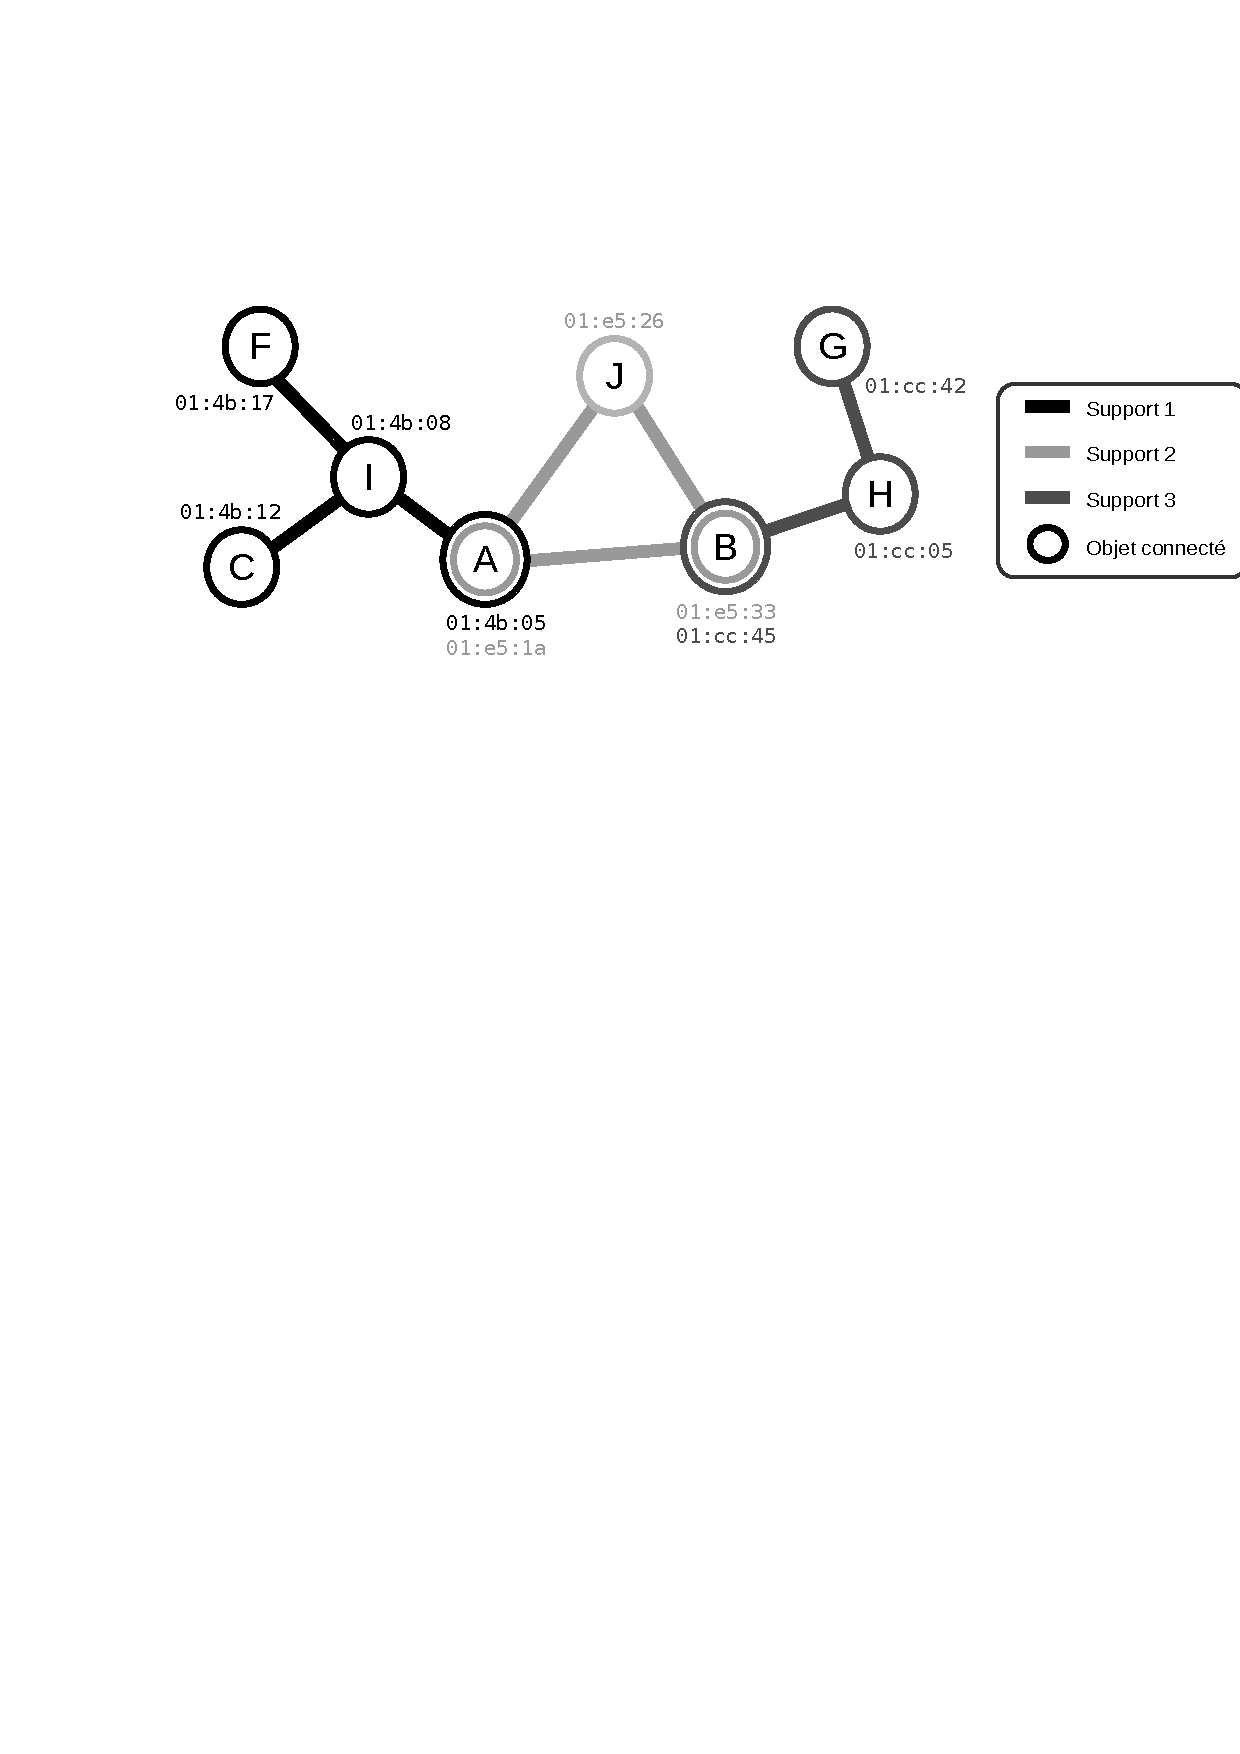
\includegraphics[width=\textwidth]{img/vip_net.png}
				\caption{Exemple de réseau en spécifiant les adresses VIP.}
				\label{vipNet}
			\end{figure}
			
			\begin{table}[!ht]
				\centering
				\begin{tabular}{|c|c|c|c|}
					\hline
					Objet              & Adresse de réseau & Passerelle        & interface \\ 
					\hline\hline
					\multirow{3}{*}{A} & \texttt{01:4b:00} & \texttt{00:00:00} & support 1 \\
					                   & \texttt{01:e5:00} & \texttt{00:00:00} & support 2 \\
					                   & \texttt{00:00:00} & \texttt{01:e5:33} & support 2 \\ \hline
					\multirow{3}{*}{B} & \texttt{01:e5:00} & \texttt{00:00:00} & support 2 \\
					                   & \texttt{01:cc:00} & \texttt{00:00:00} & support 3 \\
					                   & \texttt{00:00:00} & \texttt{01:e5:1a} & support 2 \\ \hline
					\multirow{2}{*}{C} & \texttt{01:4b:00} & \texttt{00:00:00} & support 1 \\
					                   & \texttt{00:00:00} & \texttt{01:4b:05} & support 1 \\ \hline
					\multirow{2}{*}{F} & \texttt{01:4b:00} & \texttt{00:00:00} & support 1 \\
					                   & \texttt{00:00:00} & \texttt{01:4b:05} & support 1 \\ \hline
					\multirow{2}{*}{G} & \texttt{01:e5:00} & \texttt{00:00:00} & support 3 \\
					                   & \texttt{00:00:00} & \texttt{01:cc:45} & support 3 \\ \hline
					\multirow{2}{*}{H} & \texttt{01:cc:00} & \texttt{00:00:00} & support 3 \\
					                   & \texttt{00:00:00} & \texttt{01:cc:45} & support 3 \\ \hline
					\multirow{2}{*}{I} & \texttt{01:4b:00} & \texttt{00:00:00} & support 1 \\
					                   & \texttt{00:00:00} & \texttt{01:e5:1a} & support 1 \\ \hline
					\multirow{2}{*}{J} & \texttt{01:e5:00} & \texttt{00:00:00} & support 2 \\
					                   & \texttt{00:00:00} & \texttt{01:e5:1a} & support 2 \\ \hline
				\end{tabular}
				\caption{Les tables de routage des différents objets de la figure \ref{vipNet}}
				\label{routingTable}
			\end{table}

			Comme l'on montré ces exemples, l'utilisation des tables de routage est un bon moyen pour
			transporter un message dans la totalité du réseau virtuel. Mais actuellement, elle possède
			un petit inconvénient. Il est nécessaire d'écrire les tables de routage de chacun des
			objets faisant passerelle. Il existe cependant des algorithmes de mise à jour dynamique
			des tables de routage mais ils n'ont pas encore été étudiés dans ce projet.

	\subsection{Un réseau dynamique}
		Le protocole VIP est suffisant pour mettre en place une architecture d'objets connectés dans
		une maison mais il manque cependant une étape pour que les messages puissent utiliser
		correctement les supports de communication. Imaginons que l'on souhaite envoyer un message 
		à un objet appartenant au même support. On connait on connait son adresse VIP. Mais comment 
		fait on pour déterminer à qui appartient l'adresse ? Il est en effet nécessaire de pouvoir 
		faire le lien entre l'adresse de support d'un objet et son adresse VIP. Pour cela, il a été
		mis en place un protocole nommé VARP (Virtual Address Resolution Protocol) inspiré du
		protocole ARP. Ce protocole permet d'effectuer des demandes d'adresses VIP ou d'adresses de
		support. Par exemple, si un objet est en possession d'une adresse de support, il peut
		récupérer l'adresse VIP correspondante avec une requête VARP. Et à l'inverse, il peut
		récupérer une adresse de support à partir d'une adresse VIP. Il est également possible de
		faire une requête multiple en utilisant une adresse de broadcast. Cela signifie que tous les
		objets acceptant cette adresse répondront à la requête. Cela peut par exemple être utilisé
		pour mettre à jour une table contenant la liste des couples d'adresses support/VIP des objets
		voisins. Le tableau \ref{varpEx} présente quelques exemples d'utilisation du protocole VARP.
		
		\begin{figure}[!ht]
			\centering
			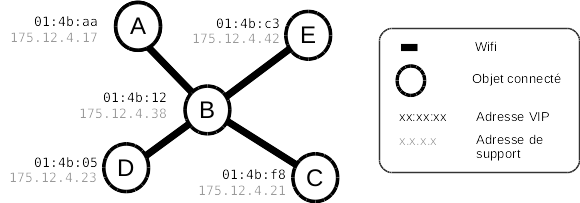
\includegraphics[width=\textwidth]{img/varp_net.png}
			\caption{Exemple de réseau Wifi d'objets connectés avec leurs adresses IP et VIP.}
			\label{varpNet}
		\end{figure}
		
		\begin{table}[!ht]
			\centering
			\begin{tabular}{|l|l|l||l|l|l|}
				\hline
				\multicolumn{3}{|c||}{Requête}     & \multicolumn{3}{|c|}{Réponse}  \\ \hline
				Objet & Demande & Adresse connue  & Objet & Adresse VIP & Adresse IP  \\ 
\hline\hline
				A     & IP      & 01:4b:f8        & C     & 01:4b:f8    & 175.12.4.21 \\ \hline
				A     & IP      & 01:4b:ff        & B     & 01:4b:12    & 175.12.4.38 \\
				      &         &                 & C     & 01:4b:f8    & 175.12.4.21 \\
				      &         &                 & D     & 01:4b:05    & 175.12.4.23 \\
				      &         &                 & E     & 01:4b:c3    & 175.12.4.42 \\ \hline
				A     & VIP     & 175.12.4.38     & B     & 01:4b:12    & 175.12.4.38 \\ \hline
				A     & VIP     & 255.255.255.255 & B     & 01:4b:12    & 175.12.4.38 \\
				      &         &                 & C     & 01:4b:f8    & 175.12.4.21 \\
				      &         &                 & D     & 01:4b:05    & 175.12.4.23 \\
				      &         &                 & E     & 01:4b:c3    & 175.12.4.42 \\ \hline
			\end{tabular}
			\caption{Exemple d'utilisation du protocole VARP par rapport à la figure \ref{varpNet}}
			\label{varpEx}
		\end{table}
		
		En faisant des scans réguliers en utilisant le protocole VARP, il est possible de détecter
		la connexion ou la déconnexion d'objets dans le réseau virtuel. Cela peut être pratique 
		pour rendre le réseau dynamique. Mais lorsqu'un nouvel objet se connecte au réseau, il faut
		cependant qu'il possède déjà une adresse VIP. De plus, cette adresse doit également respecter
		l'adresse de sous-réseau du support dans lequel il va se connecter. Sinon, il ne sera pas 
		possible de communiquer avec ce nouvel objet. La solution à ce problème serait d'affecter
		automatiquement une adresse VIP à chaque nouvel objet qui rejoint le réseau. Le protocole
		DHCP (Dynamic Host Configuration Protocol) à été conçu pour ça dans les réseaux Ethernet. Il
		faut donc créer un protocole similaire pour les objets connectés dans le réseau virtuel.
		Ce protocole n'a pas encore été étudié et n'est donc pas présent dans l'implémentation 
		actuelle du réseau virtuel.
		
		Avec la mise en place d'un système de connexion dynamique d'objets connectés, il est possible
		de mettre en place un nouveau type d'objet que l'on appelera \emph{objet mobile}. Ce genre
		d'objet doit pouvoir se déconnecter d'un sous-réseau lorsqu'il sort de sa portée mais il doit 
		également se connecter automatiquement aux réseaux qui sont dans sa proximité. Ils possèdent
		donc une adresse VIP variable. En utilisant un identifiant unique pour ces objets, il est
		possible de les localiser "grossièrement" dans la maison si l'on sait où sont placer les
		objets fixes. Cette information peut alors être utilisée pour effectuer des actions
		particulières dans des protocoles de plus haut niveau. Si l'on transforme des montres 
		intelligentes ou encore des smartphones en objet connecté, on peut alors déterminer la
		localisation d'une personne dans le réseau virtuel.
	
% 		apparition, disparition ou déplacement d’objets dans le réseau
% 		présentation du protocole VARP
% 		exemple d’apparition d’un objet
% 		les objets mobiles
%     aborder le protocole "pseudo DHCP" et expliquer qu'il n'est pas encore pensé
 
\section{La généricité des objets connectés}
	Avec les protocoles VIP et VARP, nous avons vu comment sont transportés les messages entre 
	n'importe quels objets du réseau virtuel. Il est temps maintenant de passer à un niveau plus haut
	et de s'intéresser à la composition de ces messages. 
	
	\subsection{Description d'un objet dans le protocole}
		Jusqu'à présent, tous les éléments du réseau virutel ont été décrit comme étant des objets
		connectés. On peut alors se demander pourquoi les différents noeuds du réseau sont qualifiés
		ainsi ? Quels sont leurs caractéristiques ? La définition d'un objet connecté a déjà été 
		abordé brièvement dans la première partie de ce rapport. Maintenant nous allons voir un peu
		plus en détails les fonctionnalités de ceux-ci. Tous ces éléments sont définis dans 
		un protocole encapsulé dans le protocole VIP : le protocole SDCP (Smarts Devices 
		Communication Protocol). Le tableau \ref{modeleCouche} illustre l'organisation des différentes
		couches du protocole de SmartDevCom.
		
		\begin{table}[!ht]
			\centering
			\begin{tabular}{r|c|c|c|}
				\cline{2-4}
				& & & Ethernet \\ \cline{4-4}
				Couche réseau & Bluetooth & ZigBee & IP \\ \cline{4-4}
				& & & UDP \\ \cline{2-4}
				\multirow{2}{*}{Couche réseau virtuel} & \multirow{2}{*}{VARP} & 
				\multicolumn{2}{c|}{VIP} \\ \cline{3-4}
				&                      & \multicolumn{2}{c|}{SDCP} \\
				\cline{2-4}
			\end{tabular}
			\caption{Représentation des différentes couches réseaux du protocole utilisé par 
					   SmartDevCom}
			\label{modeleCouche}
		\end{table}
		
		Le protocole permet de définir des objets connectés dont on ne connait pas la composition à 
		l'avance. Il est donc nécessaire de définir des règles permettant de décrire n'importe quel
		objet. Ce protocole doit alors essayer de rester le plus générique possible tout en offrant
		des fonctionnalités simples d'utilisation. Le protocole définit un objet connecté de la 
		manière suivante :
		\begin{itemize}
			\item il possède zéro, un ou plusieurs capteurs
			\item il possède zéro, un ou plusieurs actionneurs
			\item il possède zéro, une ou plusieurs actions
			\item il définit la façon dont doivent être utilisé chacune des actions
			\item il permet l'exécution de chacune de ses actions
		\end{itemize}
		
		Pour rappel, on considère ici qu'un capteur est un module d'un objet capable de mesurer une
		grandeur physique de son environnement. Un actionneur est un module capable d'agir sur son
		environnement. Une action représente une requête ou un ordre que l'on peut donner à un ou
		plusieurs des modules d'un objet. Étant donné que l'on ne connait pas forcément à l'avance
		à quoi correspond une action, il est nécessaire de définir précisément les paramètres qu'elle
		prend ainsi que les informations qu'elle retourne. L'ensemble des ces caractéristiques est
		récupérable à distance grâce à des requêtes définies dans le protocole SDCP. C'est justement
		cet ensemble de requêtes qui permet de pouvoir communiquer avec un objet sans avoir à
		connaitre au préalable à quoi il sert.
		
	\subsection{Méthode de classification des actions sur les objets}
% 		recherche des informations caractérisant les actions
% 		algorithmes de classification
		Pour pouvoir utiliser convenablement un objet inconnu, il est cependant nécessaire de pouvoir
		le ranger dans une certaine catégorie d'objet. En effet, on exécutera une de ses actions 
		uniquement si l'on sais à quoi elle sert. C'est pourquoir le protocole SDCP définit des types
		de capteurs, des types d'actionneurs et surtout des types d'actions. Dans cette architecture,
		connaitre le type des capteurs et des actionneurs d'un objet n'est pas quelque chose 
		d'indispensable. Lors de l'utilisation d'un objet, ce qui nous importe c'est l'exécution 
		des actions. Si l'on prend l'exemple d'un objet capable d'allumer la lumière en appuyant 
		sur un interrupteur mural. La demande de liste des actionneurs va retourner le servomoteur
		qui s'occupe de changer l'état du bouton. La demande de liste d'actions va retourner l'action
		permettant d'allumer ou d'éteindre la lumière. On remarque que le type de l'actionneur n'a
		que peu d'intérêt par rapport au type de l'action car ce dernier apporte une information bien
		plus précise.
		
		Mais le problème le plus important dans ce protocole est la définition des types des actions.
		Ce type doit valider deux contraintes : il doit définir précisément le rôle de l'action et
		il doit également être générique. Cela signifie par exemple que si un nouvel objet
		apparait dans le réseau avec un type d'action inconnu, les autres objets doivent pouvoir 
		comprendre de la façon la plus précise possible à quoi sert cette action. Cela pose demande
		donc beaucoup de réflexion sur la méthode à utiliser pour construire les types d'actions.
		
		Une solution intéressante pour résoudre ce problème serait de construire un arbre de type
		d'action. Cela permettrait de pouvoir définir des actions de façon très précise (lorsque l'on
		s'approche des feuilles de l'arbre) et également conserver un certain ordre d'idée pour 
		des types qui n'existe pas encore dans l'arbre (on connaitrait au moins l'une des branches de
		l'arbre). Mais la construction de cet arbre de type n'est, encore une fois, pas évidente.
		Pour cette construction, une première approche a été faite en utilisant des outils de
		statistique. Il existe en effet beaucoup d'algorithmes de clusterisation qui crée des
		structures sous forme d'arbre. Le problème de ces algorithmes est qu'ils utilisent des données
		quantitatives. Dans notre cas, les données sont pûrement qualitatives. Pour ce genre de
		données, une des méthodes consiste à lister un ensemble d'actions le plus varié possible et
		de rechercher des critères pouvant discriminer ces actions. Cette méthode est intéressant mais
		la recherche des critères discriminant est presque aussi compliqué que d'essayer de construire
		l'arbre des types à la main.
		
		Finalement, l'arbre des types d'actions a été écrite manuellement en essayant de faire le tour
		des types d'actions que l'on peut potentiellement rencontrer avec des objets connectés. Voici
		un extrait de la liste des types d'actions actuellement gérées (le vrai arbre est sur 4 
		niveaux) :
		\begin{itemize}
			\item ambiance
			\begin{itemize}
				\item action kinéstésique
				\item action visuelle
				\item action auditive
			\end{itemize}
			\item sécurité
			\item multimédia
			\begin{itemize}
				\item audio
				\item vidéo
			\end{itemize}
			\item électroménager
			\begin{itemize}
				\item alimentaire
			\end{itemize}
			\item accessibilité (humain)
			\begin{itemize}
				\item déplacement
				\item ouverture de porte
				\item localisation
			\end{itemize}
			\item entretien
		\end{itemize}

	\subsection{Gestion dynamique d’objets}
% 		comment un objet d’un nouveau type peut s’intégrer à la hiérarchie
% 		les différentes solutions d’intégration
% 		exemple
		Cette méthode de gestion des types d'actions est déjà suffisante pour la plupart des objets
		que l'on serait susceptible de créer. Mais il est cependant possible d'aller encore plus loin
		en créant des objets spéciaux agissant comme des bases de données. Ces objets auront pour
		tâche de mettre à jour un arbre de type regroupant tous les types que l'on peut rencontrer
		dans le réseau virtuel. Cette base sera bien évidemment dynamique pour que des nouveaux objets
		puissent ajouter de nouveau type. Ces objets peuvent également rassembler d'autres types de
		données comme par exemple la liste des actions de tous les objets. Ce regroupement
		d'informations peut être très utile pour d'autres objets dont l'unique but est de contrôler
		des objets existants.
		
		Le protocole SmartDevCom réunit assez d'outils pour pouvoir créer des objets connectés très 
		variés. Il permet d'avoir une structure solide sur laquelle on peut alors mettre en place 
		tout une hiérarchie d'objets connectés allant du simple objet appuyant sur un bouton jusqu'à
		des objets intégrant de l'intelligence artificielle et dédié au contrôle des autres objets.
		Il n'y a alors plus aucune limite dans la dynamicité et la réactivité du réseau virtuelle.

